
In recent years, large language models (LLMs) and their underlying transformer architecture~\citep{vaswani2017attention,devlin2018bert,brown2020language,ouyang2022instructgpt} have become the cornerstone of conversational AI and have led to a wide array of consumer and enterprise applications. Despite these advances, the limited fixed-length context windows used by LLMs significantly hinders their applicability to long conversations or reasoning about long documents.
For example, the most widely used open-source LLMs can only support a few dozen back-and-forth messages or 
reason about a short document 
before exceeding their maximum input length \citep{touvron2023llama2}.

Directly extending the context length of transformers incurs a quadratic increase in computational time and memory cost due to the transformer architecture's self-attention mechanism, making the design of new long-context architectures a pressing research challenge~\citep{dai2019transformerxl,kitaev2020reformer,beltagy2020longformer}. 
While developing longer models is an active area of research \citep{dong2023longcontextsurvey}, 
even if we could overcome the computational challenges of context scaling, recent research shows that long-context models struggle to utilize additional context effectively \citep{liu2023lostinmiddle}.
As consequence, given the considerable resources needed to train state-of-the-art LLMs and diminishing returns of context scaling, there is a critical need for alternative techniques to support long context. 












In this paper, we study how to provide the illusion of an infinite context while continuing to use fixed-context models.
Our approach borrows from the idea of virtual memory paging that was developed to enable applications to work on datasets that far exceed the available memory by paging data between main memory and disk.
We leverage the recent progress in function calling abilities of LLM agents \citep{schick2023toolformer,liu2023agentbench} to design \ours, an OS-inspired LLM system for \textbf{virtual context management}.
Using function calls, LLM agents can read and write to external data sources, modify their own context, and choose when to return responses to the user. 


These capabilities allow LLMs to effective  ``page'' in and out information between context windows (analogous to ``main memory" in operating systems) and external storage, similar to hierarchical memory in traditional OSes. 
In addition, function calls can be leveraged to manage control flow between context management, response generation, and user interactions. This allows for an agent to choose to \textit{iteratively} modify what is in its context for a single task, thereby more effectively utilizing its limited context. 









In \ours, we treat context windows as a constrained memory resource, and design a memory hiearchy for LLMs analogous to memory tiers used in traditional OSes \citep{patterson1988caseforraid}. 
Applications in traditional OSes interact with \textit{virtual memory}, which provides an illusion of there being more memory resources than are actually available in physical (i.e., main) memory by the OS paging overflow data to disk and retrieving data (via a page fault) back into memory when accessed by applications.
To provide a similar illusion of longer context length (analogous to virtual memory), we allow the LLM to manage what is placed in its own context (analogous to physical memory) via an `LLM OS', which we call \ours. \ours enables the LLM to retrieve relevant historical data missing from what is placed in-context, and also evict less relevant data from context and into external storage systems.
Figure~\ref{fig:system} illustrates the components of \ours.

\begin{figure}[t]
    \centering
\begin{center}
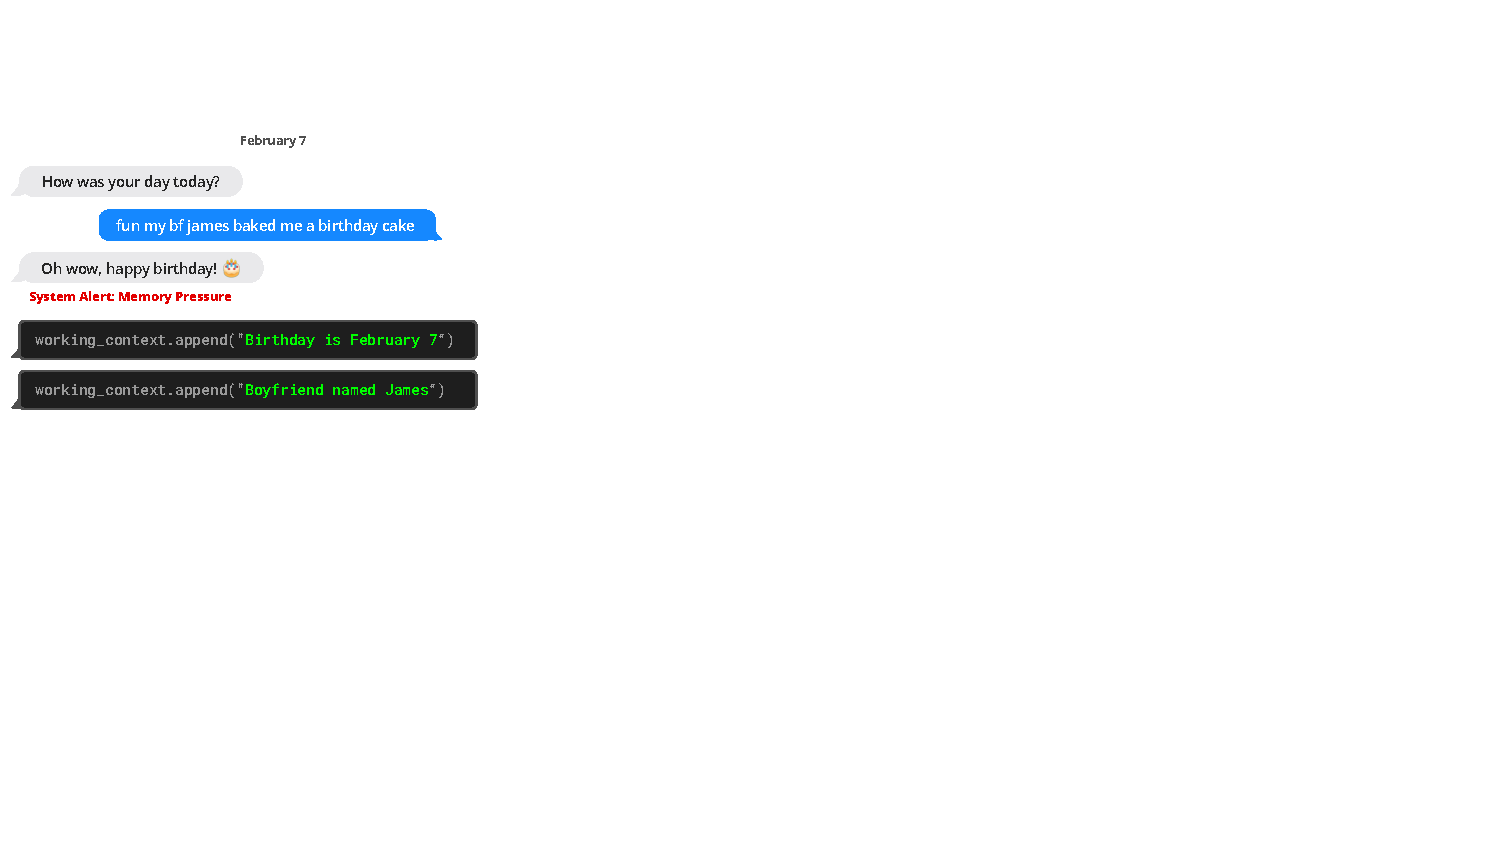
\includegraphics[width=0.45\textwidth]{images/memgpt_diagrams_wide_memory_creation.pdf}
\end{center}
    \vspace{-1.5em}
    \caption{
\ours (left) writes data to persistent memory after it receives a system alert about limited context space.
}
    \label{fig:example-memory-creation}
\end{figure}










The combined use of a memory-hierarchy, OS functions and event-based control flow allow \ours to handle unbounded context using LLMs that have finite context windows.
To demonstrate the utility of our new OS-inspired LLM system, we evaluate \ours on two domains where the performance of existing LLMs is severely limited by finite context: document analysis, where the length of standard text files can quickly exceed the input capacity of modern LLMs, and conversational agents, where LLMs bound by limited conversation windows lack context awareness, persona consistency, and long-term memory during extended conversations. 
In both settings, \ours is able to overcome the limitations of finite context to outperform existing LLM-based approaches.



\begin{figure}[t]
    \centering
\begin{center}
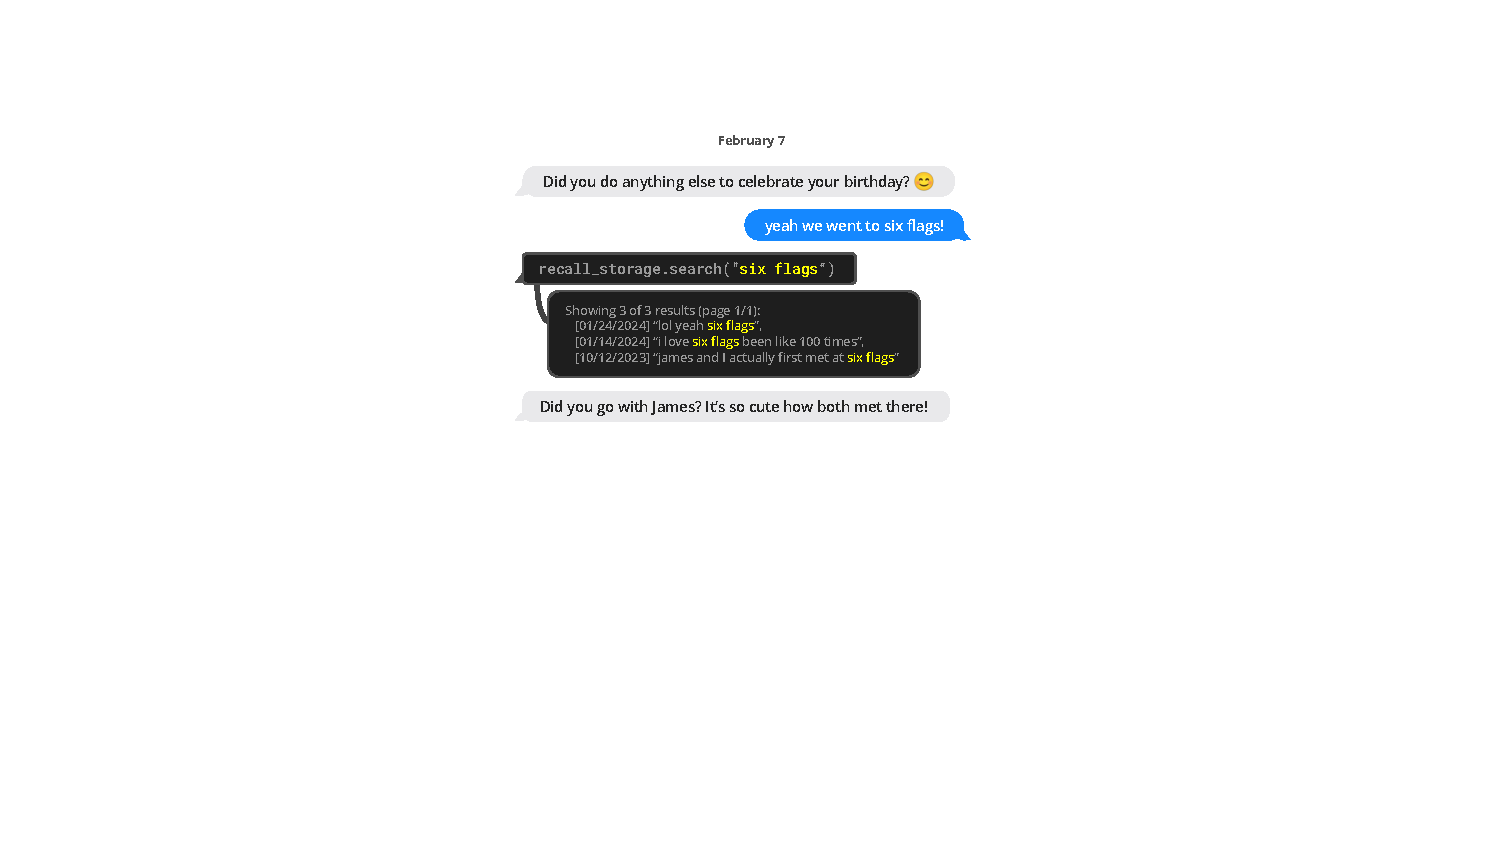
\includegraphics[width=0.45\textwidth]{images/memgpt_diagrams_wide_memory_search.pdf}
\end{center}
    \vspace{-1.5em}
    \caption{
\ours (left) can search out-of-context data to bring relevant information into the current context window.
}
    \label{fig:example-memory-search}
\end{figure}

\begin{figure*}[t!]
\begin{center}
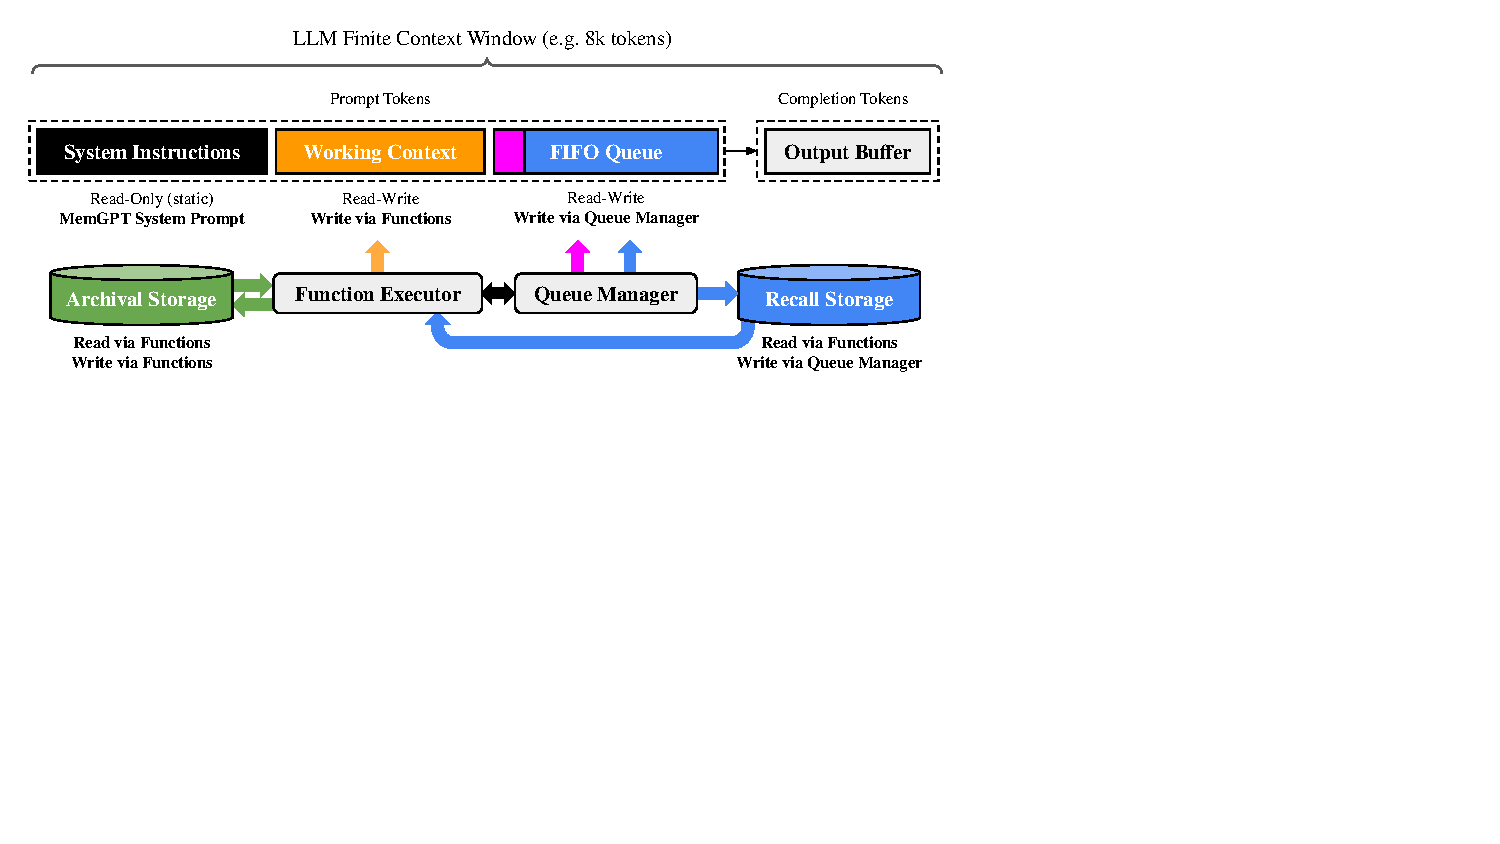
\includegraphics[width=0.885\textwidth]{images/memgpt_system_flow_2.pdf}
\end{center}
\caption{
In \ours, a fixed-context LLM processor is augmented with a hierarchical memory system and functions that let it manage its own memory.
The LLM's prompt tokens (inputs), or \emph{main context}, consist of the system instructions, working context, and a FIFO queue. 
The LLM completion tokens (outputs) are interpreted as function calls by the function executor. 
\ours uses functions to move data between main context and \emph{external context} (the archival and recall storage databases). 
The LLM can request immediate follow-up LLM inference to chain function calls together by generating a special keyword argument (\texttt{request\_heartbeat=true}) in its output; function chaining is what allows MemGPT to perform multi-step retrieval to answer user queries.
}
\label{fig:system}
\end{figure*}
